\documentclass[11pt]{article}
\usepackage{fontspec}
\usepackage[margin=1in]{geometry}
\usepackage{amsmath}
\usepackage{array,booktabs,longtable,listings}
\usepackage{placeins}
\usepackage{tikz}
\usepackage{authblk}
\usetikzlibrary{arrows.meta,positioning}
\usepackage{xurl}
\usepackage[hidelinks]{hyperref}
\newcommand{\sha}{\operatorname{SHA256}}
\setlength{\emergencystretch}{2em}

\title{Native Confidential Audit Proofs for \\
Liquid Regulated Assets}
\author{Kyrylo Riabov, Artem Chystiakov}
\affil{Blockstream}
\date{\today}

\begin{document}
    \maketitle

    \begin{abstract}
        We describe a confidential compliance construction for regulated assets on Liquid.
        Each regulated output carries a proof that allows a third-party auditor to retrospectively recover transferred amounts for regulatory reporting.
        Both fast (optimistic) and slow (bounded discrete-log) fallback methods are provided.
        The Simplicity spending program verifies the proof and asserts that the native Elements value commitment and an auditor handle use the same blinding factor.
        Holders transfer assets without issuer participation, retaining Liquid's ordinary amount confidentiality.
    \end{abstract}


    \section{Introduction}

    Liquid confidential transactions hide asset amounts from public observers while preserving ledger balance rules \cite{liquid}.
    Regulated assets, however, may need selective third-party audit and full transaction history reporting for compliance reasons.
    Native Liquid confidential transactions do not provide such functionality.
    This paper borrows the audit goal and twisted-ElGamal construction of PGC \cite{pgc}, but it does not adopt PGC's account system or its equal-value proof.
    Instead, it proves a relation over the value commitment already present in an Elements output.
    The covenant and consensus therefore check the same value commitment.

    The onchain Simplicity program verifies a native commitment proof for every regulated output \cite{simplicity}.
    The enclosing covenant authorizes the holder and enforces the asset's spending policy.
    Issuer-only recovery runs offchain and does not participate in holder transfer authorization.

    We state the audit relation, its transaction binding, recovery rules, and confidentiality limits.
    Appendix~\ref{app:code-math} gives a SimplicityHL implementation of the checks described in this paper.

    This construction may be useful to asset-management protocols such as DAMP \cite{damp-paper}.

    \section{Elements confidential-assets prerequisites}
    \label{sec:elements}

    Liquid uses Elements confidential transactions to hide amounts while allowing consensus to check transaction balance and range proofs \cite{liquid,confidential-assets}.
    Let $\mathcal{G}$ be the prime-order secp256k1 group of order $q$, with standard generator $G$.
    For an asset identifier $A$, Elements derives the asset generator
    \[
        H_A=\texttt{hash\_to\_curve}(A)\in\mathcal{G},
    \]
    whose discrete logarithm relative to $G$ is unknown.
    We write a Pedersen value commitment as $\operatorname{Com}_{H}(v,b)=vH+bG$.
    Its additive structure permits balance checks through
    \[
        \operatorname{Com}_{H}(v_1,b_1)+\operatorname{Com}_{H}(v_2,b_2)
        =\operatorname{Com}_{H}(v_1+v_2,b_1+b_2).
    \]
    A separate range proof constrains the committed amount to an integer interval
    \[
        v_{\min}\leq v\leq v_{\max},\qquad v\text{ an integer}.
    \]

    Elements can hide the asset identifier as well as the amount.
    In that general case, the asset and value blinders $a$ and $b$ give
    \[
        \widetilde H_A=H_A+aG,
        \qquad
        \widetilde C=v\widetilde H_A+bG=vH_A+(va+b)G.
    \]
    Asset surjection proofs establish the relation between input and output asset types \cite{liquid,confidential-assets}.
    Here the regulated output instead carries the explicit identifier $A$ and a confidential amount.
    The verifier requires this explicit asset field and derives the unblinded generator $H_A$ from it respectively.
    Thus the native value commitment used throughout this paper is
    \begin{equation}
        C=vH_A+bG,
        \label{eq:commitment}
    \end{equation}
    for amount $v$ and nonzero value blinder $b$.
    The regulated asset id remains public.

    A native confidential value field encodes $C=(x_C,y_C)$ as
    \[
        \operatorname{enc}_{\mathrm{native}}(C)
        =\operatorname{prefix}(y_C)\mathbin\Vert\operatorname{bytes}_{32}(x_C),
        \qquad \operatorname{prefix}(y_C)\in\{\texttt{08},\texttt{09}\}.
    \]
    The encoding occupies 33 bytes.
    These prefixes encode the quadratic character of the y-coordinate, as detailed in Appendix~\ref{app:native-sign}.
    For output index $i$, the spending program reads the actual asset and value fields and requires
    \[
        (\mathsf{asset}_i,\mathsf{value}_i)
        =\operatorname{unwrap}(\texttt{output\_amount}(i)),
        \qquad \mathsf{asset}_i=\operatorname{Explicit}(A),
    \]
    \[
        \mathsf{value}_i=\operatorname{Confidential}\bigl(\operatorname{enc}_{\mathrm{native}}(C)\bigr),
        \qquad H_A=\texttt{hash\_to\_curve}(A).
    \]
    The remaining transaction data comes from the jets \cite{simplicity-jets}:
    \[
        \begin{aligned}
            \mathsf{scriptHash}_i&=\operatorname{unwrap}(\texttt{output\_script\_hash}(i)),\\
            \mathsf{rangeProofHash}_i&=\operatorname{unwrap}(\texttt{output\_range\_proof}(i)),\\
            \mathsf{signatureDigest}&=\texttt{sig\_all\_hash}().
        \end{aligned}
    \]
    Curve jets such as \texttt{scale}, \texttt{linear\_combination\_1}, and \texttt{gej\_equiv}, together with SHA-256 jets, implement the proof equations and transcript hashing.
    Elements consensus verifies the native range proof. The additional audit checks below bind that same commitment to the issuer's audit handle.


    \section{Protocol model}
    \label{sec:model}

    \subsection{Roles and ledger objects}

    The issuer selects a nonzero audit secret $s$ and publishes
    \begin{equation}
        P=sG.
        \label{eq:audit-key}
    \end{equation}
    A sender adds the audit handle
    \begin{equation}
        D=bP.
        \label{eq:handle}
    \end{equation}
    The issuer computes
    \begin{equation}
        C-s^{-1}D=vH_A.
        \label{eq:recovery-target}
    \end{equation}
    Recovering $v$ from this point is a discrete-log search over an application range.

    The enclosing covenant must require one audit record for every regulated output and preserve the regulated asset's spending conditions.
    For audit reporting, an offchain issuer process indexes the chain from a configured provider, recovers amounts, and reconstructs the resulting state.
    Its report may be signed to authenticate the final result.

    Figure~\ref{fig:flow} shows the protocol lifecycle and the audit check.

    \begin{figure}[ht]
        \centering
        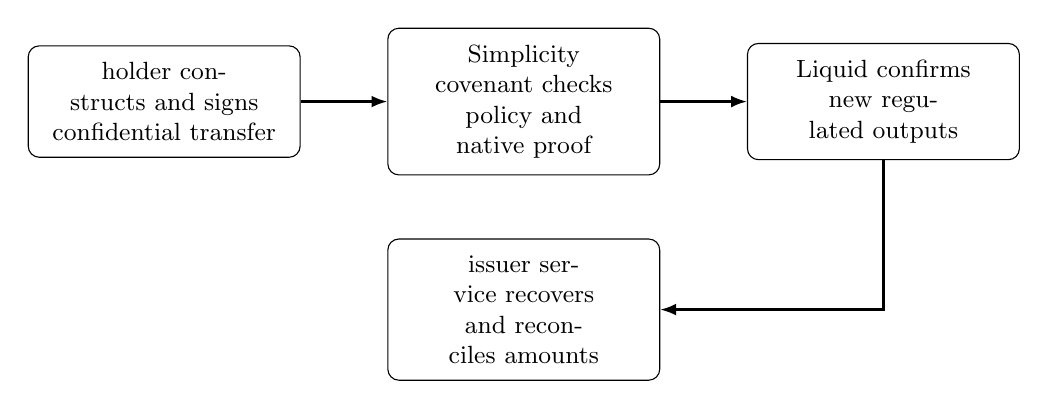
\begin{tikzpicture}[
            node distance=0.8cm and 1.1cm,
            box/.style={draw, rounded corners, align=center, font=\small, inner sep=6pt, text width=0.25\linewidth},
            arrow/.style={-{Latex[length=2mm]}, thick}
        ]
        \node[box] (holder) {holder constructs and signs\\confidential transfer};
        \node[box, right=of holder] (covenant) {Simplicity covenant checks\\policy and native proof};
        \node[box, right=of covenant] (ledger) {Liquid confirms\\new regulated outputs};
        \node[box, below=of covenant] (audit) {issuer service recovers\\and reconciles amounts};
        \draw[arrow] (holder) -- (covenant);
        \draw[arrow] (covenant) -- (ledger);
        \draw[arrow] (ledger) |- (audit);
        \end{tikzpicture}
        \caption{Holder authorization, covenant enforcement, and issuer reporting steps.}
        \label{fig:flow}
    \end{figure}


    \FloatBarrier
    \section{Native audit construction}
    \label{sec:construction}

    \subsection{Public context}
    \label{sec:statement-proof}

    Let $R$ denote the public recovery byte string defined below.
    For each regulated output, we collect its public context in
    \begin{equation}
        \Gamma=(d,g,e,P,h,i,A,C,S,\sha(R)).
        \label{eq:statement}
    \end{equation}
    The deployment parameters are the 32-byte audit-domain salt $d$, a fixed domain word $g=2$ that identifies this transcript domain, the audit epoch $e$, and the issuer's audit public key $P$.
    The transaction binding is its \texttt{sig\_all\_hash}, denoted $h$.
    The remaining fields identify the output: $i$ is its index, $A$ the regulated asset, $C$ the native value commitment, and $S$ the output script hash.
    Appendix~\ref{app:code-math} identifies the compiled parameters and their encodings.
    The complete public statement is $(\Gamma,D)$, since the proof also exposes the audit handle $D$.
    The secret witness is the output opening $(v,b)$ satisfying
    \[
        C=vH_A+bG \quad\text{and}\quad D=bP.
    \]
    The proof links the ledger commitment and the audit handle to one blinder without revealing the amount or blinder to the verifier.

    \subsection{Recovery record and its hash}
    \label{sec:recovery-record}

    An honestly constructed record lets the issuer recover $(v,b)$ by decryption instead of searching for $v$ in Equation~\ref{eq:recovery-target}.
    An honest sender chooses a fresh ephemeral secret $k$, publishes $E=kG$, and derives an encryption key $K$ from ECDH with $P$.
    The issuer obtains the same shared secret because $sE=kP$.
    AES-256-GCM-SIV encrypts the 40-byte opening $\operatorname{BE}_8(v)\mathbin\Vert\operatorname{BE}_{32}(b)$ under $K$ and a fresh 12-byte nonce $N$.
    Here $\operatorname{BE}_j$ denotes a fixed-width, $j$-byte big-endian integer encoding.

    We write $\operatorname{SEC1}(Q)$ for the compressed point encoding specified in \emph{Standards for Efficient Cryptography 1: Elliptic Curve Cryptography}, abbreviated SEC~1 \cite[Section~2.3.3]{sec1}.
    For a finite secp256k1 point $Q=(x_Q,y_Q)$, this is a 33-byte string: the prefix byte \texttt{02} for even $y_Q$ or \texttt{03} for odd $y_Q$, followed by $\operatorname{BE}_{32}(x_Q)$.
    The curve equation and this parity bit determine $y_Q$, so the sender does not need to transmit the full y-coordinate.
    This encoding differs from the native Elements commitment encoding of $C$, whose prefixes \texttt{08} and \texttt{09} are explained in Appendix~\ref{app:native-sign}.
    The current 102-byte record is
    \[
        R=\underbrace{\mathtt{01}}_{1\ \mathrm{byte}}
        \mathbin\Vert\underbrace{\operatorname{SEC1}(E)}_{33\ \mathrm{bytes}}
        \mathbin\Vert\underbrace{N}_{12\ \mathrm{bytes}}
        \mathbin\Vert\underbrace{\mathrm{ciphertext}\mathbin\Vert\mathrm{tag}}_{40+16\ \mathrm{bytes}}.
    \]
    The leading byte selects the recovery-envelope format.
    Associated data binds $d,e,i,A,C,S$ to the encryption.
    It excludes $h$.
    The sender first constructs $R$, commits the ordered recovery records in the transaction's final \texttt{OP\_RETURN}, computes $h$, and only then produces the native proof.
    This order avoids a circular dependency between the ciphertext and the transaction digest.

    All of $R$ is public, but an observer without the audit secret sees ciphertext rather than the opening.
    The covenant hashes the exact 102 bytes and includes $\sha(R)$ in the proof challenge.
    It does not decrypt them or prove that the ciphertext contains $(v,b)$.
    An all-zero record denotes missing auxiliary data.
    Even missing or invalid recovery bytes can accompany a valid native proof, provided those exact bytes were committed when that proof was made.
    Replacing $R$ afterwards changes the challenge and the transaction's recovery commitment.
    Binding the record prevents substitution but does not guarantee successful recovery.
    Section~\ref{sec:recovery} explains the issuer's decryption checks and bounded fallback.

    \subsection{Proof messages and challenge}
    \label{sec:proof-messages}
    The prover samples $\alpha,\beta\overset{\$}{\leftarrow}\mathbf{Z}_q^{*}$ independently and uniformly at random and publishes
    \begin{align}
        T_C &= \alpha H_A+\beta G, & T_D &= \beta P. \label{eq:nonce-commitments}
    \end{align}
    These are fresh proof commitments.
    Their nonce scalars are distinct from the encryption secret $k$ and nonce $N$ inside $R$.
    The prover retries if $T_C$ is the point at infinity, since transmitted points use finite SEC~1 encodings.
    It derives the challenge $c$ by BIP-340-style tagged SHA-256 over the encoded context, $D$, $T_C$, and $T_D$, reduced modulo $q$ \cite{bip340}:
    \[
        c=\operatorname{int}\!\left(
                                  \operatorname{TaggedHash}_{\tau}
                                  \bigl(\operatorname{enc}(\Gamma)\mathbin\Vert\operatorname{SEC1}(D)
                                  \mathbin\Vert\operatorname{SEC1}(T_C)\mathbin\Vert\operatorname{SEC1}(T_D)\bigr)
        \right)\bmod q.
    \]
    The fixed domain-separation tag is \texttt{DAMP/audit/v2}.
    The encoding uses the field order in Equation~\ref{eq:statement}, fixed-width integers, the native Elements encoding of $C$, and a fixed output-role byte \texttt{00} immediately before $\sha(R)$.
    Appendix~\ref{app:code-math} gives the exact byte order and corresponding source lines.
    The responses are
    \begin{align}
        z_v&=\alpha+cv\pmod q, & z_b&=\beta+cb\pmod q. \label{eq:responses}
    \end{align}
    The algebraic proof is $(D,T_C,T_D,z_v,z_b)$.
    The verifier reconstructs $\Gamma$, checks canonical point and scalar encodings, recomputes $c$, and checks
    \begin{align}
        z_vH_A+z_bG &= T_C+cC, \label{eq:verify-commitment}\\
        z_bP &= T_D+cD. \label{eq:verify-handle}
    \end{align}

    \paragraph{Why Equations~\ref{eq:verify-commitment} and \ref{eq:verify-handle} hold.}
    Scalar multiplication distributes over addition, and all scalar arithmetic is modulo the group order $q$.
    Substituting the responses from Equation~\ref{eq:responses} gives
    \begin{align*}
        z_vH_A+z_bG
        &= (\alpha+cv)H_A+(\beta+cb)G\\
        &= (\alpha H_A+\beta G)+c(vH_A+bG)\\
        &= T_C+cC,\\[3pt]
        z_bP
        &= (\beta+cb)P\\
        &= \beta P+c(bP)\\
        &= T_D+cD.
    \end{align*}
    The first equality checks the opening of $C$.
    The second links its blinder to $D$ through the same response $z_b$.
    This proves completeness: an honest prover with the stated opening satisfies both verification equations.
    It does not by itself prove an amount interval, successful decryption of $R$, or chain inclusion.

    For the underlying interactive protocol, two accepting transcripts for the same $(\Gamma,D,T_C,T_D)$ and distinct challenges $c,c'$ yield
    \[
        v=(z_v-z'_v)(c-c')^{-1}\pmod q,\qquad
        b=(z_b-z'_b)(c-c')^{-1}\pmod q.
    \]
    Subtracting the two verification equations shows that these extracted values satisfy both relations.
    The inverse exists because $q$ is prime and $c\ne c'$.
    The construction uses the noninteractive Fiat--Shamir transform, so its knowledge claim is in the random-oracle model and depends on the usual transform assumptions \cite{faust-fiat-shamir}.
    This algebraic argument has not received an independent cryptographic audit.

    \subsection{Binding to the spend}

    The covenant reconstructs the statement from transaction data and its compiled deployment parameters.
    Binding to \texttt{sig\_all\_hash} commits the proof to the finalized transaction.
    The explicit output index prevents moving a record between outputs.
    Asset, commitment, script hash, deployment, domain word, and epoch prevent reuse across assets, destinations, transcript domains, deployments, or audit-key epochs.
    Hashing the recovery bytes prevents an intermediary from replacing the issuer's recovery record while retaining the proof.

    Recovery must authenticate these fields from the transaction and its witness.
    It must re-execute the actual covenant witness, extract one canonical audit-record witness, check the native range-proof profile, rebuild the statement from the transaction, and verify Equations~\ref{eq:verify-commitment} and \ref{eq:verify-handle}.
    Chain inclusion must be checked separately.

    The Simplicity program in Appendix~\ref{app:code-math} supports at most ten regulated inputs and ten regulated outputs per transfer.
    Audit records use 4,096 Simplicity budget words.
    These limits are operational constraints, not security arguments.

    \subsection{Amount interval}

    We use an application amount interval from $1$ through $2^{63}-1$ base units.
    The covenant accepts the endpoint $2^{63}$ because the pinned native range-proof header and commitment binding establish that interval.
    The Sigma relation alone does not establish a range.
    If recovery yields $v=2^{63}$, it flags the amount as exceeding the application's maximum of $2^{63}-1$, even though the covenant accepts that endpoint.
    That being said, we recommend issuance total supply up to $2^{56}$ sats.

    \section{Recovery and confidentiality}
    \label{sec:recovery}

    \subsection{Authenticated fast path}

    The sender encrypts $(v,b)$ to the audit public key with ephemeral ECDH and AES-256-GCM-SIV.
    Associated data commits to the deployment, epoch, output index, asset, native commitment, and output script.
    After decryption, recovery recomputes $C$ and $D$ and verifies the native proof before presenting the amount.

    The recovery ciphertext is a fast path, not a transfer-validity condition.
    A missing, unsupported, or unauthenticated record does not invalidate a transfer whose native proof and covenant witness are valid.
    Transfer validity does not depend on the issuer being online.
    It also means complete recovery is not guaranteed when a sender withholds valid auxiliary data.

    \subsection{Bounded fallback}

    If the fast path fails, the issuer can use Equation~\ref{eq:recovery-target} and search for $v$ in a bounded interval.
    Table~\ref{tab:dlog-64} reproduces Table~6 of \emph{Discrete Logarithm Solvers on secp256k1: Algorithms and Benchmark Results}, dated August~24, 2026 \cite{dlog-benchmark}.
    The source benchmarks secrets in $[0,2^{64})$ against $G$ with a range containing the native range-proof interval $[1,2^{63}]$.
    Recovery here uses $H_A$, so any precomputed table must use that asset generator.
    The reported timings are external benchmark results, not measurements of this audit construction.

    \begin{table}[htbp]
        \centering
        \footnotesize
        \setlength{\tabcolsep}{3pt}
        \renewcommand{\arraystretch}{1.15}
        \caption{Discrete log solver benchmark - 64-bit secrets (100 secrets per algorithm). Reproduced from Table~6 of \cite{dlog-benchmark}.}
        \label{tab:dlog-64}
        \begin{tabular}{@{}>{\raggedright\arraybackslash}p{.27\linewidth}p{.22\linewidth}rrrrr@{}}
            \toprule
            Algorithm & Table & Size & Solved & Best & Average & Worst \\
            \midrule
            BSGS & \multicolumn{6}{p{.70\linewidth}@{}}{skipped - BSGS tables only go up to 32 bits} \\
            NaiveLookup & \multicolumn{6}{p{.70\linewidth}@{}}{skipped - reuses a doubled-size BSGS table, capped at 16-bit secrets} \\
            BSGS-k64 & \multicolumn{6}{p{.70\linewidth}@{}}{skipped - BSGS-k tables only go up to 32 bits} \\
            BSGS-k1024 & \multicolumn{6}{p{.70\linewidth}@{}}{skipped - BSGS-k tables only go up to 32 bits} \\
            NaiveDoubledLookup & \multicolumn{6}{p{.70\linewidth}@{}}{skipped - reuses a doubled-size BSGS-k table, capped at 16-bit secrets} \\
            TBSGS-k64 & \multicolumn{6}{p{.70\linewidth}@{}}{skipped - TBSGS-k tables only go up to 32 bits} \\
            TBSGS-k1024 & \multicolumn{6}{p{.70\linewidth}@{}}{skipped - TBSGS-k tables only go up to 32 bits} \\
            NaiveTruncated\linebreak[0]DoubledLookup & \multicolumn{6}{p{.70\linewidth}@{}}{skipped - reuses a doubled-size TBSGS-k table, capped at 16-bit secrets} \\
            BL12 & generated (19090.181~s) & 7.0~MiB & 84/100 & 1.437~s & 243.071~s & 593.449~s \\
            \bottomrule
        \end{tabular}
    \end{table}

    ``Table'' records generation or cache use, ``Size'' is serialized table size, and ``Solved'' counts successful solves out of 100.
    BL12 was the only tested variant that ran at 64 bits.
    The skipped BSGS variants store table indices as 16-bit integers and cap their secret range at 32 bits. The naive variants reuse tables at twice their secret width and therefore stop at 16 bits.
    These are limits of the tested software, not fundamental limits of those algorithms.

    BL12 table generation took 19090.181 seconds, about 5 hours 18 minutes.
    Each solve had a 600-second timeout: 84 of 100 instances completed and 16 timed out.
    Best, Average, and Worst cover only the 84 successes and exclude all 16 timeouts.
    The reported 243.071-second average therefore understates the mean cost of a solve attempt, and the worst successful solve, 593.449 seconds, nearly reaches the timeout.
    The source describes BL12 as a randomized Las Vegas algorithm with an unbounded runtime tail.
    Its testing-environment section is unfilled, so the hardware and toolchain are unspecified.
    A timeout leaves the amount unknown.
    These results do not guarantee complete recovery, so a lesser bound of 56 bits is recommended.

    \subsection{What remains confidential}

    Public observers see the ordinary Liquid transaction fields, the native commitment, the audit handle, the proof, and the recovery bytes.
    The issuer can recover an amount because it knows $s$ or can decrypt the auxiliary record.
    For parties without that secret, amount privacy is computational.
    It relies on the hiding of Elements commitments, DDH-type hardness for the linked handle, honest-verifier zero knowledge of the underlying Sigma relation and the Fiat--Shamir model, plus ECDH and authenticated-encryption security for the recovery record \cite{pgc,faust-fiat-shamir}.
    We do not give a new security reduction that combines these assumptions.

    This paper does not prove universal payment confidentiality.
    Transaction structure, fees, scripts, timing, input and output counts, and queried transaction identifiers remain observable.
    Reporting through a public explorer API reveals queried identifiers to the provider.
    A private Elements node is required when that access pattern is sensitive.

    \section{Audit key rotation}

    Audit key rotation remains unresolved in this paper.

    \section{Security considerations}
    \label{sec:security}

    A successful holder spend has a native audit proof for each regulated output, tied to the transaction.
    Leaking the audit secret, Equation~\ref{eq:recovery-target} removes the value blinder, making the amount permanently visible to everyone.

    Production use needs a sharper key-custody design, independent review of the cryptography and Simplicity checks, side-channel analysis, longer-lived indexing, provider diversity, and operational recovery procedures.

    \section{Conclusion}

    The construction connects selective audit to the native Liquid value commitment and enforces that relation in the Simplicity spending path.
    Holders authorize transfers without issuer participation, while the issuer can recover amounts through authenticated decryption or bounded discrete-log search.

    The appendix gives the SimplicityHL checks and their mathematical correspondence.
    The external 64-bit benchmark illustrates both the cost and the timeout risk of discrete-log recovery when authenticated recovery data is unavailable.
    A 56-bit asset total supply bound is recommended.


    \section*{AI disclosure}

    Parts of this work were prepared with AI assistants.
    The assistants helped analyze source material, draft the paper, and review the SimplicityHL code under the authors' direction.
    The authors reviewed the generated content and take responsibility for the final result.

        {\small\sloppy
    \bibliographystyle{unsrt}
    \bibliography{references}
    }

    \appendix
    \clearpage
\section{Simplicity-to-mathematics correspondence}
\label{app:code-math}

This appendix maps the native audit verifier in the reference implementation to Section~\ref{sec:construction}.
The source is \href{https://github.com/BlockstreamResearch/damp/blob/d48f1833c5a5663ed2de48dfb2f7d762a9f3d19c/simf/lib/audit.simf}{\texttt{simf/lib/audit.simf}} at revision \texttt{d48f183}.
The numbered listings include that module directly.
The tables explain each source statement and group multiline statements together.
Blank lines have no semantic role; the tables group declaration delimiters with their enclosing statement.
The \texttt{.simf} files are SimplicityHL source compiled into the Simplicity programs executed by the covenant.
This is a source-level correspondence, not a machine-checked equivalence proof.

\lstdefinestyle{auditcode}{
  basicstyle=\ttfamily\fontsize{8.5}{10}\selectfont,
  numbers=left, numberstyle=\tiny, numbersep=8pt,
  xleftmargin=1.8em, frame=tb, columns=fullflexible,
  breaklines=true, breakatwhitespace=false, keepspaces=true,
  showstringspaces=false, tabsize=4, aboveskip=9pt, belowskip=9pt
}
\newcommand{\auditlisting}[2]{%
  \lstinputlisting[style=auditcode,firstline=#1,lastline=#2,firstnumber=#1]{../../simf/lib/audit.simf}%
}
\newcommand{\auditmap}[2]{\texttt{#1} & #2\\}
\newenvironment{auditmapping}{%
  \begingroup\small
  \renewcommand{\arraystretch}{1.12}%
  \begin{longtable}{@{}>{\raggedright\arraybackslash}p{.12\linewidth}>{\raggedright\arraybackslash}p{.85\linewidth}@{}}
  \toprule
  Source lines & Mathematical meaning or check\\
  \midrule
  \endhead
  \bottomrule
  \endfoot
}{%
  \end{longtable}\endgroup
}

\subsection{Notation and point encoding}

Several source names differ from the paper's symbols.
The local variable \texttt{c} is the point $C$, while \texttt{e} is the challenge $c$.
The local \texttt{h} is $H_A$, not the transaction digest $h$.
The argument \texttt{d} is $D$, not the deployment salt $d$; the salt and audit epoch come from \texttt{AUDIT\_DEPLOYMENT} and \texttt{AUDIT\_EPOCH}.
The variable \texttt{aux} holds $R$, and \texttt{root} is a field element $\rho$ used only to authenticate the native commitment's sign.

Write a compressed curve point as $(\eta,x_C)$, where $\eta$ is the SEC~1 parity bit defined in Section~\ref{sec:statement-proof}.
\texttt{Ge} denotes an affine point and \texttt{Gej} a Jacobian point.
The pair \texttt{(point, 1)} embeds an affine point with Jacobian coordinate $Z=1$.
\texttt{gej\_equiv} compares represented group elements, not their raw Jacobian coordinates.
The curve's base-field prime is $p_F=2^{256}-2^{32}-977$, distinct from the scalar order $q$.

\auditlisting{1}{19}
\begin{auditmapping}
  \auditmap{1-3}{State the module's purpose and import checked counter addition/subtraction. These imports do not implement a group equation.}
  \auditmap{5-6}{Declare \texttt{point\_ge} and unpack a compressed point into its parity bit and $x$ coordinate.}
  \auditmap{7}{Require $0\leq x<p_F$ by equality with field normalization. Reject a noncanonical coordinate.}
  \auditmap{8}{Decompress the curve point selected by $(\eta,x)$; \texttt{unwrap} rejects a non-point. This establishes a finite point on secp256k1.}
  \auditmap{9}{End the point-decoding helper.}
  \auditmap{11-12}{Declare \texttt{hash\_point} and unpack the point to serialize into a SHA-256 state.}
  \auditmap{13}{Select the SEC~1 prefix from parity.}
  \auditmap{14}{An even $y$ coordinate uses byte \texttt{02}.}
  \auditmap{15}{An odd $y$ coordinate uses byte \texttt{03}.}
  \auditmap{16}{Complete prefix selection.}
  \auditmap{17}{Append the one-byte SEC~1 prefix to the transcript.}
  \auditmap{18}{Append the 32-byte $x$ coordinate, completing $\operatorname{SEC1}(Q)$ for the supplied point $Q$.}
  \auditmap{19}{End the serialization helper.}
\end{auditmapping}

\subsection{Read the native commitment and validate proof fields}
\label{app:native-sign}

\auditlisting{21}{54}
\begin{auditmapping}
  \auditmap{21-31}{Declare the verifier with output index $i$, SEC~1 parity $\eta$, sign witness $\rho$, points $D,T_C,T_D$, responses $z_v,z_b$, and digest $\sha(R)$. These are public proof or encoding data, not $(v,b)$.}
  \auditmap{32}{Read the actual asset and amount field of output $i$ from the transaction. Reject a missing output.}
  \auditmap{33}{Require an explicit asset identifier, not an asset commitment.}
  \auditmap{34}{Require that identifier to equal the compiled regulated asset $A$.}
  \auditmap{35}{Require a confidential value commitment and unpack its native sign bit $\epsilon$ and coordinate $x_C$. Reject an explicit amount.}
  \auditmap{36}{Decode a candidate $C=(x_C,y_C)$ using the supplied SEC~1 parity $\eta$.}
  \auditmap{37}{Read its $y_C$ coordinate for the native-sign check.}
  \auditmap{39-40}{Document why the native Elements sign bit must not be interpreted as SEC~1 parity.}
  \auditmap{41}{Require the witness $\rho$ to be a canonical field element.}
  \auditmap{42}{Select a quadratic-residue target from the native sign bit.}
  \auditmap{43}{For prefix \texttt{08}, require a square root of $y_C$.}
  \auditmap{44}{For prefix \texttt{09}, require a square root of $-y_C$.}
  \auditmap{45}{Complete the target selection.}
  \auditmap{46}{Check $\rho^2=(-1)^\epsilon y_C\pmod {p_F}$. This ties the decoded point to the actual native encoding of $C$.}
  \auditmap{47}{Derive $H_A$ with the Elements asset-generator jet \texttt{hash\_to\_curve}.}
  \auditmap{48}{Read the compiled audit public key $P$.}
  \auditmap{49}{Decode $P$ as a canonical finite curve point.}
  \auditmap{50}{Decode the proof's handle $D$.}
  \auditmap{51}{Decode the proof commitment $T_C$.}
  \auditmap{52}{Decode the proof commitment $T_D$.}
  \auditmap{53}{Require $0\leq z_v<q$. Reject a noncanonical scalar encoding.}
  \auditmap{54}{Apply the same canonical-scalar check to $z_b$.}
\end{auditmapping}

The native prefixes \texttt{08} and \texttt{09} distinguish the quadratic character of $y_C$.
They do not mean even and odd $y_C$.
For secp256k1, $p_F\equiv3\pmod4$, so $-1$ is a quadratic nonresidue.
For nonzero $y_C$, exactly one of $y_C$ and $-y_C$ has a square root.
A finite point in this odd-prime-order group cannot have $y_C=0$.
Thus line 46 accepts only the sign selected by the native prefix, even though line 36 starts from a separately supplied SEC~1 parity bit.
Changing $C$ to $-C$ while retaining the same native commitment bytes fails this sign check.
The prover derives the witness $\rho$ from public curve coordinates; it does not reveal the opening of $C$.

\subsection{Construct the Fiat--Shamir challenge}

Let $t=\sha(\mathtt{DAMP/audit/autonomous/v3})$.
The challenge uses $\sha(t\mathbin\Vert t\mathbin\Vert m)$ with
\begin{align*}
 m={}&d\mathbin\Vert\operatorname{BE}_4(2)\mathbin\Vert\operatorname{BE}_8(e)
       \mathbin\Vert\operatorname{SEC1}(P)\mathbin\Vert h\mathbin\Vert\operatorname{BE}_4(i)\\
    &\mathbin\Vert\operatorname{asset}(A)\mathbin\Vert\operatorname{native}(C)
       \mathbin\Vert S\mathbin\Vert\mathtt{00}\mathbin\Vert\sha(R)\\
    &\mathbin\Vert\operatorname{SEC1}(D)\mathbin\Vert\operatorname{SEC1}(T_C)
       \mathbin\Vert\operatorname{SEC1}(T_D).
\end{align*}
Here $\operatorname{asset}(A)$ is the 32-byte consensus-order asset identifier, not its display-order hexadecimal text.
The encoding $\operatorname{native}(C)$ consists of the native prefix \texttt{08} or \texttt{09} and $x_C$, for 33 bytes in total.
The fixed role byte \texttt{00} is part of the transcript even though it is not a variable in $x$.
The \texttt{v3} tag names the challenge format; it does not change the domain word $g=2$.

\auditlisting{56}{84}
\begin{auditmapping}
  \auditmap{56-57}{Document the ordered domain and transaction fields.}
  \auditmap{58}{Start a SHA-256 context.}
  \auditmap{59-61}{Append $t$, whose hexadecimal value is the source constant.}
  \auditmap{62-64}{Append $t$ again, implementing the tagged-hash prefix $t\mathbin\Vert t$.}
  \auditmap{65}{Append the 32-byte deployment salt $d$.}
  \auditmap{66}{Append $\operatorname{BE}_4(g)$ with $g=2$.}
  \auditmap{67}{Append the 8-byte audit epoch $e$.}
  \auditmap{68}{Append $\operatorname{SEC1}(P)$.}
  \auditmap{69}{Append the introspected transaction digest $h=\texttt{sig\_all\_hash()}$.}
  \auditmap{70}{Append the 4-byte output index $i$.}
  \auditmap{71}{Append the 32-byte consensus asset identifier $A$.}
  \auditmap{72}{Select the native commitment prefix using the bit read from the transaction.}
  \auditmap{73}{Use \texttt{08} when $y_C$ is a quadratic residue.}
  \auditmap{74}{Use \texttt{09} when $y_C$ is a quadratic nonresidue.}
  \auditmap{75}{Complete the native-prefix selection.}
  \auditmap{76}{Append that one-byte native prefix.}
  \auditmap{77}{Append $x_C$, completing the transaction's exact 33-byte native commitment.}
  \auditmap{78}{Append $S=\sha(\mathrm{scriptPubKey}_i)$ from transaction introspection.}
  \auditmap{79}{Append the fixed output-role byte \texttt{00}.}
  \auditmap{80}{Append $\sha(R)$, calculated from the record bytes in lines 149-150 below.}
  \auditmap{81}{Append $\operatorname{SEC1}(D)$.}
  \auditmap{82}{Append $\operatorname{SEC1}(T_C)$.}
  \auditmap{83}{Append $\operatorname{SEC1}(T_D)$.}
  \auditmap{84}{Finalize SHA-256 and reduce its big-endian integer modulo $q$ to obtain challenge $c$. The source calls this scalar \texttt{e}.}
\end{auditmapping}

\subsection{Check the two group equations}

\noindent\begin{minipage}{\linewidth}
\auditlisting{86}{96}
\end{minipage}
\begin{auditmapping}
  \auditmap{86-87}{State the common-blinder relation and its two verification equations in source notation.}
  \auditmap{88}{Start the group-equality assertion for Equation~\ref{eq:verify-commitment}.}
  \auditmap{89}{\texttt{linear\_combination\_1} computes $z_vH_A+z_bG$. The generator $G$ is implicit in this jet.}
  \auditmap{90}{\texttt{scale} computes $cC$ and \texttt{gej\_ge\_add} adds $T_C$, giving $T_C+cC$.}
  \auditmap{91}{Require the two group elements to be equal, completing Equation~\ref{eq:verify-commitment}.}
  \auditmap{92}{Start the assertion for Equation~\ref{eq:verify-handle}.}
  \auditmap{93}{Compute $z_bP$, reusing the same response $z_b$ as line 89.}
  \auditmap{94}{Compute $cD$ and add $T_D$, giving $T_D+cD$.}
  \auditmap{95}{Require equality, completing Equation~\ref{eq:verify-handle}.}
  \auditmap{96}{Return only after both assertions succeed.}
\end{auditmapping}

The substitution proof in Section~\ref{sec:statement-proof} explains why honest responses pass these exact operations.
Neither assertion decrypts $R$, verifies a native range proof, or proves that this transaction was confirmed.

\subsection{Serialize recovery bytes and bind the native range proof}

\auditlisting{98}{130}
\begin{auditmapping}
  \auditmap{98}{Represent $R$ as $64+32+4+2=102$ bytes. This tuple splits raw bytes for SHA-256 jets; its boundaries are not the encryption-envelope field boundaries.}
  \auditmap{99}{Represent the range-proof body as $79\cdot64+4=5060$ bytes. The ten-byte header is fixed separately.}
  \auditmap{100}{Define one record as $(i,\eta,\rho,D,T_C,T_D,z_v,z_b,R,\mathrm{rangeBody})$. It contains no plaintext witness $(v,b)$.}
  \auditmap{101}{Allocate ten optional record slots, the output bound used by the verifier.}
  \auditmap{102}{Define fold state as the accepted count, previous index, finished flag, and recovery-manifest hash context.}
  \auditmap{104-105}{Declare \texttt{add\_aux} and unpack the four byte segments of $R$.}
  \auditmap{106}{Append bytes 0 through 63 of $R$.}
  \auditmap{107}{Append bytes 64 through 95 of $R$.}
  \auditmap{108}{Append bytes 96 through 99 of $R$.}
  \auditmap{109}{Append bytes 100 and 101 of $R$. Integers retain their fixed-width big-endian encoding.}
  \auditmap{110}{Return the hash context after all 102 bytes, without decoding the envelope.}
  \auditmap{112-114}{Define \texttt{range\_chunk}, which appends one 64-byte range-proof body chunk.}
  \auditmap{116-119}{Declare the range-binding check. Elements consensus verifies the range proof; this code authenticates the required profile.}
  \auditmap{120}{Unpack the 79 chunks and four-byte tail.}
  \auditmap{121}{Start a fresh SHA-256 context for the complete range proof.}
  \auditmap{122}{Append header bytes \texttt{60 3e}, selecting exponent zero and 63 mantissa bits.}
  \auditmap{123}{Append the eight-byte minimum value 1. Together the fixed header specifies $1\leq v\leq2^{63}$.}
  \auditmap{124}{Append all 79 body chunks in order.}
  \auditmap{125}{Append the final four bytes, completing the 5070-byte proof serialization.}
  \auditmap{126}{Begin a digest-equality assertion.}
  \auditmap{127}{Finalize the hash of the header and supplied body.}
  \auditmap{128}{Read the actual output range-proof hash by introspection.}
  \auditmap{129}{Require the hashes to agree, so a different body or profile cannot be substituted without a SHA-256 collision.}
  \auditmap{130}{End the range-binding helper. The Sigma equations do not replace consensus range-proof verification.}
\end{auditmapping}

The auxiliary tuple's 64-byte first segment crosses the envelope's ciphertext boundary.
The contract treats all segments as bytes.
It commits even unsupported or invalid recovery envelopes without checking whether they can be decrypted.

\subsection{Require one record per output and commit the ordered records}

For the accepted ordered records $(i_1,R_1),\ldots,(i_n,R_n)$, define
\[
 M=\sha\!\left(
   \operatorname{BE}_4(i_1)\mathbin\Vert R_1\mathbin\Vert\cdots
   \mathbin\Vert\operatorname{BE}_4(i_n)\mathbin\Vert R_n
   \mathbin\Vert\operatorname{BE}_4(n)\right).
\]
The final transaction output must have script bytes $\mathtt{6a20}\mathbin\Vert M$.
These are \texttt{OP\_RETURN}, a 32-byte push, and $M$.
This transaction-level commitment is distinct from the per-proof digest $\sha(R_j)$.

\auditlisting{132}{176}
\begin{auditmapping}
  \auditmap{132-133}{Declare the per-slot fold and unpack $(n,\mathrm{previous},\mathrm{finished},\mathrm{manifest})$.}
  \auditmap{134}{Select an empty or present record slot.}
  \auditmap{135}{An empty slot marks the list finished without changing its count or hash.}
  \auditmap{136-137}{Enter a present record and document the ordering requirement.}
  \auditmap{138}{Check whether an empty slot has already occurred.}
  \auditmap{139}{Reject a present record after a gap.}
  \auditmap{140}{Allow a record while the list remains contiguous.}
  \auditmap{141}{Complete the no-gap assertion.}
  \auditmap{142}{Unpack $(i,\eta,\rho,D,T_C,T_D,z_v,z_b,R,\mathrm{rangeBody})$.}
  \auditmap{143}{Authenticate the native range-proof profile of output $i$.}
  \auditmap{144}{Require $i>0$, excluding the verifier anchor at output zero.}
  \auditmap{145}{Inspect the previously accepted output index.}
  \auditmap{146}{The first present record has no predecessor constraint.}
  \auditmap{147}{Otherwise require $i_{j-1}<i_j$, rejecting duplicates and reordered records.}
  \auditmap{148}{Complete the predecessor check.}
  \auditmap{149-150}{Compute $\sha(R)$ over exactly the 102 witness bytes. This is the digest passed into Equation~\ref{eq:statement}.}
  \auditmap{151}{Reconstruct the statement and verify Equations~\ref{eq:verify-commitment} and \ref{eq:verify-handle} for this output.}
  \auditmap{152}{Append the four-byte index $i_j$ to the manifest context.}
  \auditmap{153}{Append $R_j$ to that same context.}
  \auditmap{154}{Increase $n$ by one with checked addition and retain $i_j$ as the predecessor.}
  \auditmap{155-157}{Return the updated state and close the branch and per-slot helper.}
  \auditmap{159}{Declare the complete record check with the expected regulated-output count.}
  \auditmap{160-161}{Fold all ten slots from count zero, no predecessor, an unfinished list, and an empty hash context.}
  \auditmap{162}{Require $n>0$.}
  \auditmap{163}{Require the number of accepted records to match the regulated-output summary. Each accepted record names a distinct actual regulated commitment.}
  \auditmap{165-166}{Document the transaction-level recovery commitment and the offchain decryption boundary.}
  \auditmap{167}{Append the four-byte count $n$ after all ordered $(i_j,R_j)$ pairs.}
  \auditmap{168}{Finalize $M$.}
  \auditmap{169}{Start hashing the required script with bytes \texttt{6a20}.}
  \auditmap{170}{Append $M$, so the expected script hash is $\sha(\mathtt{6a20}\mathbin\Vert M)$.}
  \auditmap{171}{Select the last output using checked subtraction of one from the output count.}
  \auditmap{172}{Begin the final script-hash equality check.}
  \auditmap{173}{Read the actual last output's script hash.}
  \auditmap{174}{Finalize the expected script hash.}
  \auditmap{175}{Require equality, binding the ordered recovery bytes and their count to the transaction.}
  \auditmap{176}{Return after all record and manifest checks succeed.}
\end{auditmapping}

The coverage argument also uses the caller's output scan.
In \texttt{simf/lib/assets.simf}, lines 45-60, each confidential regulated output contributes one to that scan; an explicit output contributes its positive explicit value.
In \texttt{simf/verifier/core.simf}, lines 77-108, the scan requires a positive contribution and an owner-bound script for every regulated output.
Let $J_c$ and $J_e$ be the confidential and explicit regulated-output sets.
The summary is $|J_c|+\sum_{i\in J_e}v_i$.
The record checks enforce distinct indices in $J_c$, so $n\leq|J_c|$.
Equality at line 163 therefore forces $J_e$ to be empty and every member of $J_c$ to have exactly one accepted record.
The variable names containing \texttt{amount} in the shared scan must not be read as recovered confidential balances.

\subsection{Reachability from the spending program}

The depth-four entrypoint below calls the shared audit module after checking the anchor, input policy proofs, and output scripts.
The depth-five and depth-six entrypoints have the same audit call at line 24, each using its own policy-proof verifier.
These line numbers refer to \texttt{simf/verifier\_d4.simf}, not the shared audit module.

\lstinputlisting[style=auditcode,firstline=1,lastline=25,firstnumber=1]{../../simf/verifier_d4.simf}
\begin{auditmapping}
  \auditmap{1-2}{Document the entrypoint and import the shared \texttt{verify\_records} function.}
  \auditmap{3-11}{Import transaction-shape, counting, and budget helpers.}
  \auditmap{12}{Select the depth-four policy-proof checker.}
  \auditmap{14}{Enter the SimplicityHL spending program.}
  \auditmap{15}{Consume the fixed 4096-word witness padding, requiring zero words. This is an execution-budget device, not a Sigma equation.}
  \auditmap{16}{Check input/output zero as the verifier anchor and bind the initiating holder input to its owner.}
  \auditmap{17}{Scan regulated inputs and count those that need policy proofs; do not decrypt their amounts.}
  \auditmap{18-21}{Check the supplied input policy proofs with a bounded ten-slot fold.}
  \auditmap{22}{Require every regulated input to have been checked.}
  \auditmap{23}{Check regulated output scripts and obtain the summary used by the coverage argument above.}
  \auditmap{24}{Pass \texttt{witness::AUDIT\_RECORDS} to the shared verifier. This reaches the range, statement, two-equation, and manifest checks.}
  \auditmap{25}{End the entrypoint only after all checks succeed.}
\end{auditmapping}

\subsection{Operations outside Simplicity}

\begin{samepage}
The prover computes $C=vH_A+bG$, $D=bP$, $T_C,T_D$ and $z_v,z_b$ offchain.
The covenant checks their equations onchain at the lines identified above; the prover does not supply the secret scalars.
The Rust module \texttt{damp-core::native\_audit::proof} in the reference implementation constructs and rechecks these proof messages \cite{pgc-implementation}.
\end{samepage}

The recovery module's \texttt{AuditOutput::seal} constructs $R$ using ephemeral ECDH and authenticated encryption.
\texttt{VerifiedAuditProof::open\_recovery} decrypts it with the issuer key, then checks the recovered opening against both $C$ and $D$.
Neither operation appears in the Simplicity listing.
Likewise, \texttt{recover\_bounded} computes Equation~\ref{eq:recovery-target} and searches offchain:
\[
 C-s^{-1}D
 =vH_A+bG-s^{-1}(bsG)
 =vH_A.
\]
The inverse $s^{-1}$ is a scalar inverse modulo $q$ and exists for a nonzero audit secret.
The equation removes the blinder but does not solve the discrete logarithm for $v$.
Elements consensus verifies native range proofs, and the chain-validation/reporting layer checks chain inclusion.
The appendix does not attribute either guarantee to the two Sigma assertions.

\end{document}
